\section{課題1}\label{section:kadai1}
\begin{itembox}{課題1}
2 クラス($\omega$1,$\omega$2)の識別問題を考える.データは 2 次元とする.配布するデータセットの説明を以下に示す.

\begin{itemize}
  \item Train1.txt,Train2.txt:$\omega$1,$\omega$2 に属する訓練データ集合.各データ数 50.
  \item Test1.txt,Test2.txt: $\omega$1,$\omega$2 に属するテストデータ集合.各データ数 20.
\end{itemize}

2 クラスで,2 次元のデータに対するウィドロー・ホフのアルゴリズムを実装し,訓練データから分離超平面を
学習せよ.また,テストデータの識別率(全テストデータ数に対する正しく識別されたテストデータ数の比率)を
求めよ.さらに,訓練データ,テストデータ,学習された識別面を図示せよ.
\end{itembox}
ウィドロー・ホフのアルゴリズムを初期の重みはランダムとし, 
指定した回数だけ繰り返し重みの更新を行うように実装した. 

2次元の訓練データ100件を用いて識別器の学習を行い, 40件のテストデータで
性能を測定したところ, 0.875という結果が出た. 

また, 訓練データ, テストデータのそれぞれ2クラスと識別面を図示したものが
図\ref{fig:kadai1}である. 

\begin{figure}[htbp]
  \centering
  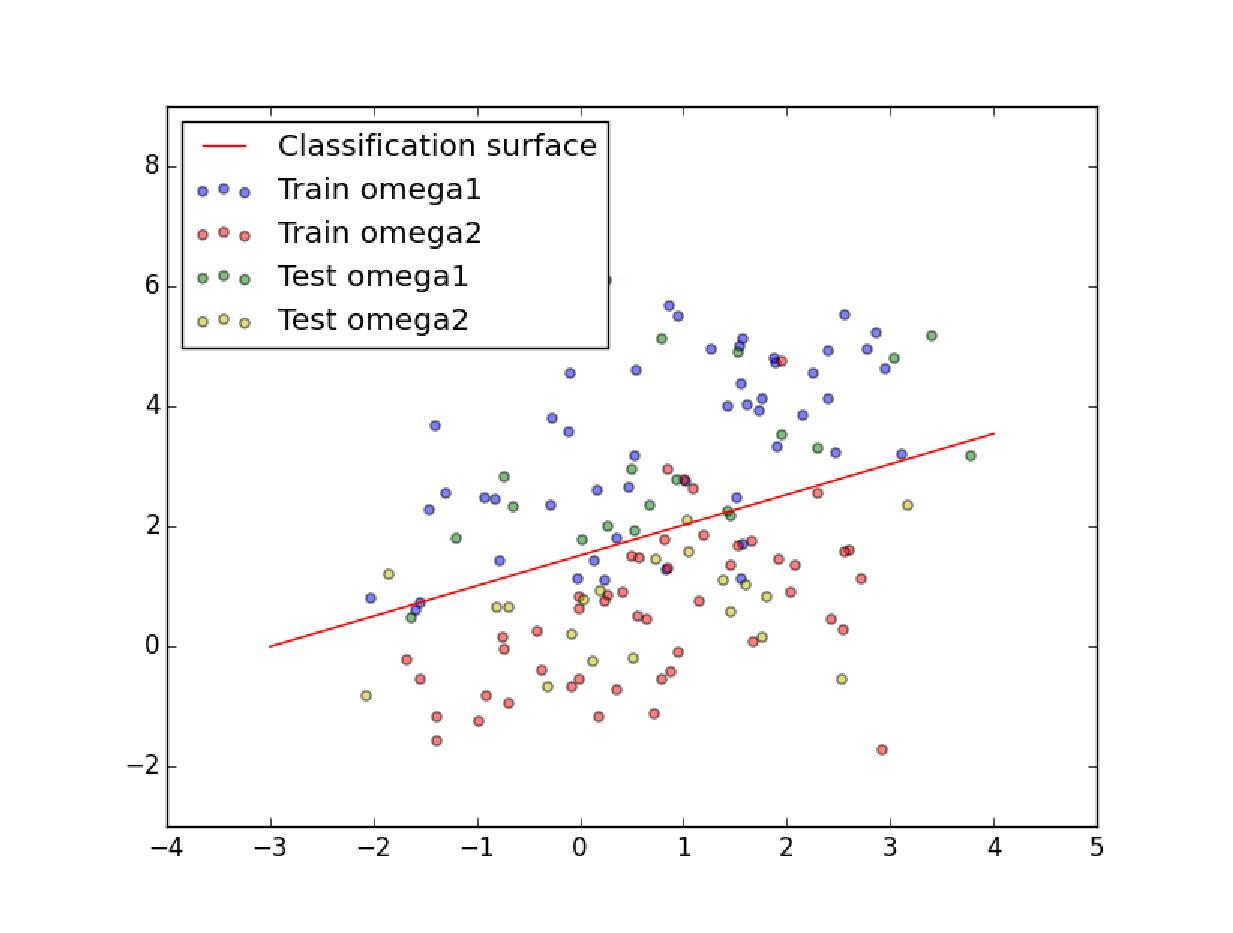
\includegraphics[width=0.7\textwidth]{./assets/kadai1_plot_20150122_031552.eps}
  \caption{データおよび識別面}
  \label{fig:kadai1}
\end{figure}

